% ----------------------------------------------------------
% Desenvolvimento
% ----------------------------------------------------------
\chapter{Resultados}\label{cap:resultados}
% ----------------------------------------------------------

Os experimentos realizados para verificar o desempenho do balanceador foram realizados em ambiente real, de maneira dinâmica através da execução dos três módulos da aplicação. Foram alocados três servidores do tipo t2.micro como servidores, um servidor t2.medium para alocar a aplicação de balanceamento e um computador para executar a aplicação para executar as requisições, no qual é armazenado o log das requisições. 
\begin{figure}[htb]
	\caption{\label{fig:tests} \textit{Screenshot} Aplicação para testar o balanceador}
	\begin{center}
		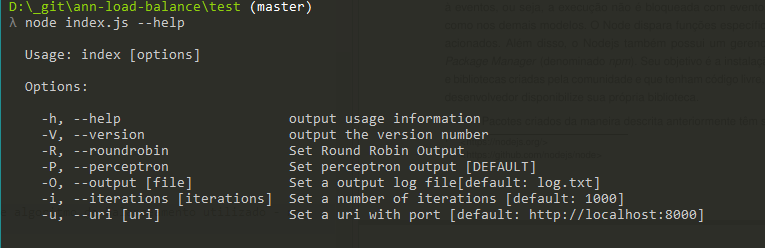
\includegraphics[width=0.70\textwidth]{img/testeapp.png}
	\end{center}
	\legend{Fonte: elaborada pela autora}
\end{figure}
Definiu-se um total de 100 requisições para avaliar o desempenho do balanceador com a Rede Neural. Para realizar os testes foi implementado uma aplicação na qual seleciona-se o tipo de algoritmo de balanceamento utilizado - no caso, a RNA ou Round Robin puro - número de iterações e url onde está hospedado o servidor de balanceamento (Figura \ref{fig:tests}). Esta aplicação armazena um arquivo de log com as informações de todas as requisições enviadas e as respostas (incluindo o servidor que atendeu a requisição). 

A avaliação do desempenho da aplicação de balanceamento foi comparada ao balanceamento realizado com Round Robin puro, através da análise dos arquivos de log gerados em ambos os casos de teste, com o mesmo número de requisições com o qual foi testada a aplicação de RNA. É fato que a aplicação de balanceamento teve desempenho satisfatório, visto que conseguiu distribuir a carga das requisições entre os servidores com sucesso, sem apresentar uma diferença significativa em relação ao algoritmo de Round Robin puro. 

Durante o processo foi possível notar que a característica que mais influenciou o processo de escolha foi a quantidade de requisições associadas ao servidor. Percebe-se também que servidores do mesmo tipo tendem a deixar o balanceamento mais equilibrado. 

A tabela \ref{tab:results} apresenta a quantidade de requisições atribuídas a cada um dos $k$ servidores alocados após executar 100 iterações na aplicação que gera requisições. Nos testes, os $k=3$ servidores são tipo t2.micro. A comparação é feita entre o balanceamento realizado com Round Robin, com a RNA sem treinamento e com a RNA após o aprendizado dos pesos.  

\begin{table}[ht]
	\caption{Comparação entre Distribuição de requisições entre servidores}
	\centering
	\begin{tabular}{c c c c}
		\hline 
		Servidores & Round Robin & RNA & RNA - treinada\\ 
		\hline 
		Servidor 1 & 34 & 36 & 37 \\ 
		\hline 
		Servidor 2 & 35 & 35 & 37 \\ 
		\hline 
		Servidor 3 & 34 & 36 & 32 \\ 
		\hline 
	\end{tabular} \\
	\vspace{3mm}
	\legend{Elaborado pela autora.}
	\label{tab:results}
\end{table}

É possível notar que não há diferença significativa entre os dois algoritmos, em relação à atribuir requisições de forma desigual. Na última coluna da tabela, nota-se que o Servidor 3 recebeu um número menor de requisições, em relação aos demais. Isto pode ter ocorrido devido à oscilações na rede. As Figuras \ref{fig:resultann}, \ref{fig:resultann2} e \ref{fig:resultrr} apresentam \textit{screenshots} dos testes. 

\begin{figure}[htb]
	\caption{\label{fig:resultann} \textit{Screenshot} Teste com RNA}
	\begin{center}
		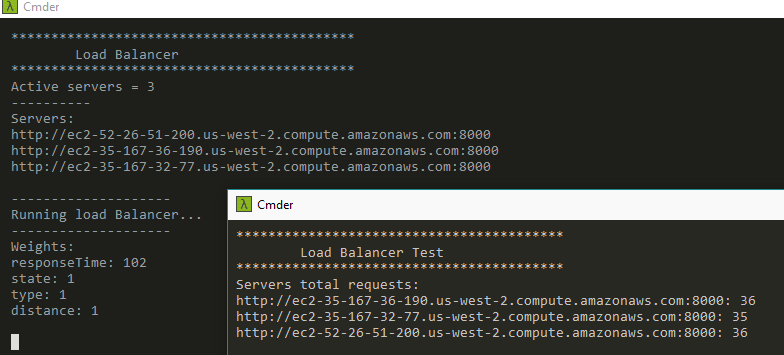
\includegraphics[width=0.70\textwidth]{img/resquisicao-ann.png}
	\end{center}
	\legend{Fonte: elaborada pela autora}
\end{figure}
\begin{figure}[htb]
	\caption{\label{fig:resultann2} \textit{Screenshot} Teste com RNA já treinada}
	\begin{center}
		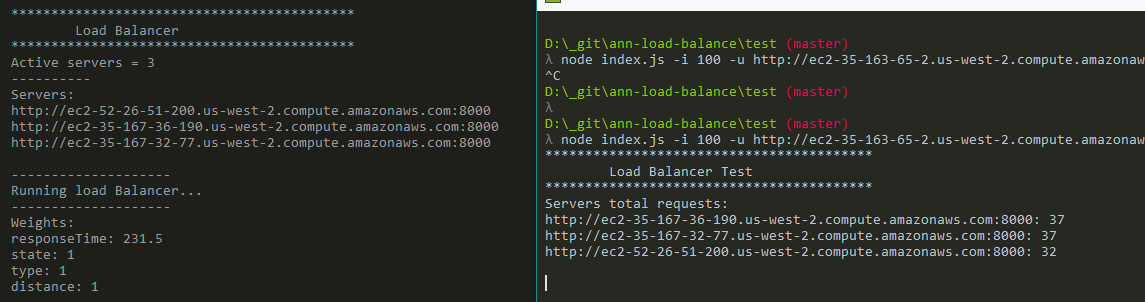
\includegraphics[width=0.90\textwidth]{img/resquisicao-ann-second.png}
	\end{center}
	\legend{Fonte: elaborada pela autora}
\end{figure}

\vspace{-10cm}

\begin{figure}[htb]
	\caption{\label{fig:resultrr} \textit{Screenshot} Teste com Round Robin}
	\begin{center}
		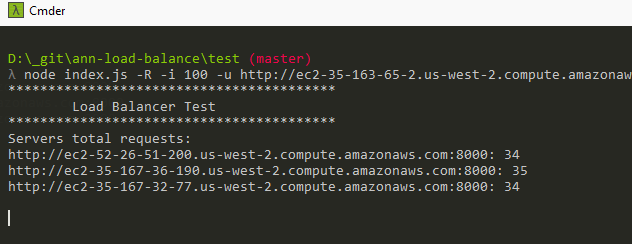
\includegraphics[width=0.70\textwidth]{img/resquisicao-round.png}
	\end{center}
	\legend{Fonte: elaborada pela autora}
\end{figure}
% ----------------------------------------------------------
